% http://blog.bemoko.com/2009/07/01/automated-mobile-web-testing-with-canoo-webtest-were-impressed/
%
\subsubsection{Canoo WebTest}
Auch Canoo WebTest ist ein auf HtmlUnit basierendes
Java-Test-Framework für Web-Applikationen. Im Gegensatz zu JWebUnit
werden die Testfälle jedoch als Ant-Tasks definiert:
\begin{lstlisting}[language=xml,
  morekeywords={project,property,import,target,webtest,config,steps,invoke,verifyTitle,setInputField,clickButton,verifyTitle}]
<project name="SimpleTest" basedir="." default="wt.full">

  <property name="webtest.home"
            location="/usr/local/java/webtest-3.0" />
  <import file="${webtest.home}/webtest.xml"/>

    <!-- runs start page test -->
    <target name="wt.testInWork"
        description="executes start page test case">

      <webtest
         name="check that WebTest is Google's top result">
	<config summary="true" />
	<steps>
	  <invoke url="http://www.google.com/ncr"
		  description="Go to Google (in English)"/>
	  <verifyTitle text="Google" />
	  <setInputField name="q" value="WebTest" />
	  <clickButton label="I'm Feeling Lucky" />
	  <verifyTitle text="Canoo WebTest Homepage" />
	</steps>
      </webtest>
    </target>
</project>
\end{lstlisting}
Ausgeführt werden diese Tests mit der Anweisung:
\begin{lstlisting}
  webtest -f web-test.xml
\end{lstlisting}
Webtest ist auch in der Lage übersichtliche Testreports zu generieren:
\begin{figure}[H]
  \centering
  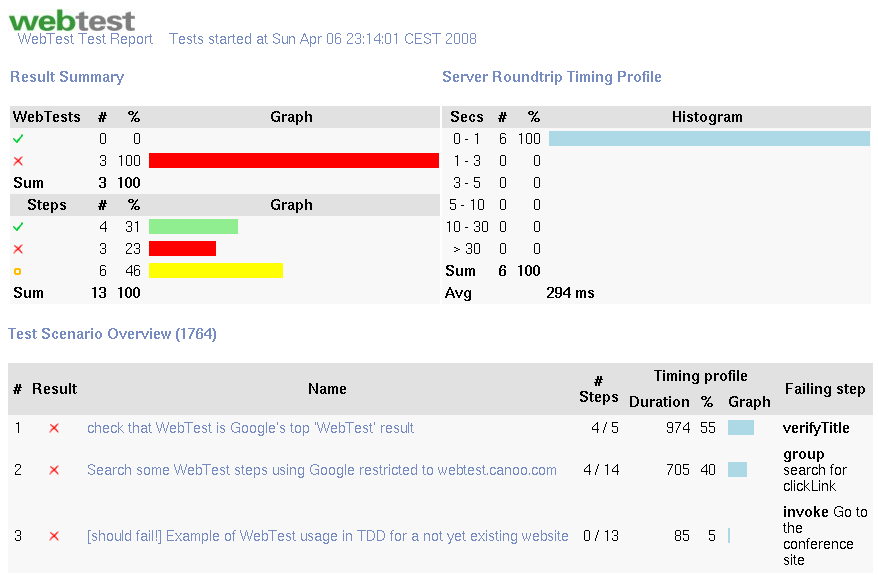
\includegraphics[width=0.8\linewidth]{qm/canoo-webtest-report}
  \caption{Canoo Webtest Report}
  \label{fig:canoo-webtest}
\end{figure}
Man kann Webtest auch in einem Maven-Projekt verwenden:
%allerdings muss zur Zeit das Plugin von Siegfrid Goeschl's Web-Seite
%
%\href{http://people.apache.org/~sgoeschl/download/maven-plugins/webtest-maven-plugin}
%  {people.apache.org/~sgoeschl/download/maven-plugins/webtest-maven-plugin}
%
%herunter geladen
% und eigenhändig im Maven-Repository installiert werden:
%
% Siehe:
% http://mguillem.wordpress.com/2009/04/30/webtest-with-groovy-maven-and-eclipse/
%
% ant -f /usr/local/java/webtest/webtest.xml wt.createProject
%
\begin{lstlisting}[language=xml,
  morekeywords={plugin,groupId,artifactId,configuration,host,port,haltonfailure,haltonerror,loglevel,executions,execution,phase,goals,goal}]
  <plugin>
    <groupId>org.codehaus.mojo</groupId>
    <artifactId>webtest-maven-plugin</artifactId>
    <configuration>
      <host>localhost</host>
      <port>8080</port>
    </configuration>
    <executions>
      <execution>
        <phase>integration-test</phase>
          <goals>
	    <goal>test</goal>
	  </goals>
	</execution>
      </executions>
  </plugin>
\end{lstlisting}
Das Plugin erwartet die webtest.xml-Datei im Verzeichnis
src/test/webtest.

Eine gutes Beispiel dazu findet man bei
Matt Raibles AppFuse-Framework \href{http://appfuse.org}{appfuse.org},
welches auch ganz allgemein beim Kick-Starting von Web-Projekten
ungemein nützlich ist.
%
% weitere beispiele:
%
% http://www.philliprhodes.com/content/testing-drupal-grails-webtest
% http://weblogs.java.net/blog/felipegaucho/archive/2009/11/18/testing-pdf-files-canoo-webtest-and-maven2
%
%
%\begin{lstlisting}[language=xml]
% <dependencies>
%     ...
%     <dependency>
%         <groupId>com.canoo.webtest</groupId>
%         <artifactId>webtest</artifactId>
%         <version>3.1-SNAPSHOT</version>
%     </dependency>
% </dependencies>
% ...
% <repositories>
%     <repository>
%         <id>webtest-dependencies-snapshot</id>
%         <name>WebTest dependencies</name>
%         <url>http://webtest.canoo.com/webtest/m2-repo-snapshots</url>
%     </repository>
% </repositories>
% \end{lstlisting}
